\documentclass{article}

\usepackage{tikz}
\usetikzlibrary{shapes,arrows}
\begin{document}

\centering
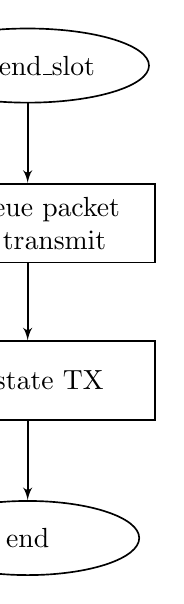
\begin{tikzpicture}[node distance = 2cm, auto, trim left, semithick]
    \tikzstyle{terminator} = [ellipse, draw,
    text width=4.5em, text centered, inner sep=6pt]
  \tikzstyle{decision} = [diamond, draw,
    text width=5em,text centered, node distance=3cm, inner sep=0pt, aspect=2]
  \tikzstyle{block} = [rectangle, draw, text width=3cm, text centered, minimum width=3cm,
    minimum height=1cm]
  \tikzstyle{line} = [draw, -latex']

  % Place nodes
  \node [terminator, text width=5em] (init) {on end\_slot};

  \node [block, below of=init] (tx) {dequeue packet and transmit};
  \node [block, below of=tx] (settx) {set state TX};

  \node [terminator, below of=settx] (end) {end};

  % Draw edges
  \path [line] (init) -- (tx);
  \path [line] (tx) -- (settx);
  \path [line] (settx) -- (end);

\end{tikzpicture}

\end{document}
